\documentclass[oneside,11pt,openright]{report}

\usepackage[latin1]{inputenc}
\usepackage[american]{babel}
\usepackage{a4}
\usepackage{latexsym}
\usepackage{amssymb}
\usepackage{amsmath}
\usepackage{epsfig}
\usepackage[T1]{fontenc}
\usepackage{lmodern}
\usepackage[labeled]{multibib}
\usepackage{color}
\usepackage{datetime}
\usepackage{epstopdf} 

\renewcommand*\ttdefault{txtt}
\newcommand{\BigO}[1]{\ensuremath{\operatorname{O}\left(#1\right)}}
\newcommand{\BigT}[1]{\ensuremath{\Theta\left(#1\right)}}

% see http://imf.au.dk/system/latex/bog/

\begin{document}

%%%%%%%%%%%%%%%%%%%%%%%%%%%%%%%%%%%%%%%%%%%%%%%%%%%%%%%%%%%%%%%%%%%%%%%

\pagestyle{empty} 
\pagenumbering{roman} 
\vspace*{\fill}\noindent{\rule{\linewidth}{1mm}\\[4ex]
{\Huge\sf Something about Computer Science}\\[2ex]
{\huge\sf Karsken B�lg, 20051234}\\[2ex]
\huge\sf Karsken B�lg, 20051234}\\[2ex]
\noindent\rule{\linewidth}{1mm}\\[4ex]
\noindent{\Large\sf Master's Thesis, Computer Science\\[1ex] 
\monthname\ \the\year  \\[1ex] Advisor: Anders M�ller\\[15ex]}\\[\fill]}
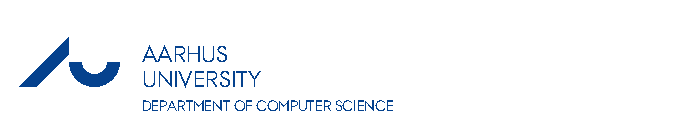
\epsfig{file=logo.eps}\clearpage

%%%%%%%%%%%%%%%%%%%%%%%%%%%%%%%%%%%%%%%%%%%%%%%%%%%%%%%%%%%%%%%%%%%%%%%

\tableofcontents
\pagenumbering{arabic}
\setcounter{secnumdepth}{2}

%%%%%%%%%%%%%%%%%%%%%%%%%%%%%%%%%%%%%%%%%%%%%%%%%%%%%%%%%%%%%%%%%%%%%%%

\chapter{Introduction}

needs content

\chapter{Binary heaps}

needs content

\section{Binary heap with array}

needs content

\section{Implementing decrease key}

needs content

\section{Time-complexity for binary heap with array}

\section{Binary heap with pointers}

needs content

\section{Implementing decrease key}

needs content

\section{Time-complexity for binary heap with pointers}

\section{Testing correctness of Binary Heaps}

needs content

\chapter{Fibonacci heaps}

In this chapter we focus on Fibonacci heaps, which is a data structure that has a forest of rooted trees as opposed to a binary heap that only has one tree ~\cite{FT87}. The data structure was invented by Michael L. Fredman and Robert Endre Tarjan and was published in the Journal of ACM in 1989. It has it name because the size of any subtree in a Fibonacci heap will be lower bounded by $F_{k+2}$ where $k$ is the degree of the root and $F$ is the Fibonacci function. Below is the time-complexities of each of the heap operations listed:

\begin{center}
  \begin{tabular}{ l | c | c | c }
    Operation & 2 Binary heap & Fibonacci heap v1 & Fibonacci heap v2 \\ \hline
    MakeHeap & $\BigT{1}$ & $\BigT{1}$ \\ 
    FindMin & $\BigT{1}$ & $\BigT{1}$ & $\BigO{\lg n}$\\ 
    Insert & $\BigT{\lg n}$ & $\BigO{1}$ \\ 
    DeleteMin & $\BigT{\lg n}$ & $\BigO{\lg n}$ & $\BigT{1}$  \\ 
    DecreaseKey & $\BigT{\lg n}$ & $\BigO{1}$ & $\BigO{1}$ \\ 
    Delete & $\BigT{\lg n}$ & $\BigO{\lg n}$ & $\BigT{1}$ \\ 
    Meld & $\BigT{n}$ & $\BigT{1}$ & $\BigT{1}$ \\
  \end{tabular}
\end{center}


\section{Fibonacci heap version 1}


\section{Worst case time-complexity for fib-v1}

needs content

\section{Fibonacci heap version 2}

needs content

\section{Worst case time-complexity for fib-v2}

needs content

\section{Testing correctness of Fibonacci Heaps}

needs content

\chapter{Test-results}

needs content

\chapter{Dijkstra}

needs content

\chapter{Binary heap vs Fibonacci heap}

needs content

\chapter{Test-results}

needs content

\chapter{Conlusion}

needs contents


%%%%%%%%%%%%%%%%%%%%%%%%%%%%%%%%%%%%%%%%%%%%%%%%%%%%%%%%%%%%%%%%%%%%%%%

\addcontentsline{toc}{chapter}{Bibliography}
\bibliographystyle{plain} 
\bibliography{report}

\end{document}

